\documentclass[accentcolor=tud0b,12pt,paper=a4]{tudreport}

\usepackage[utf8]{inputenc}
\usepackage{ngerman}
\usepackage{parcolumns}
\usepackage{verbatim}
\usepackage{hyperref}

\newcommand{\titlerow}[2]{
	\begin{parcolumns}[colwidths={1=.15\linewidth}]{2}
		\colchunk[1]{#1:} 
		\colchunk[2]{#2}
	\end{parcolumns}
	\vspace{0.2cm}
}

\title{Open Diabetes UAM Heuristik Algorithm}
\subtitle{Pflichtenheft UAM}
\subsubtitle{%
	\titlerow{Gruppe 11}{%
		Aino Schwarte <aino.schwarte@stud.tu-darmstadt.de>\\
		Anna Mees <anna.mees@stud.tu-darmstadt.de>\\
		Jan Paul Petto <janpaul.petto@stud.tu-darmstadt.de>\\
		Paul Wolfart <paul.wolfart@stud.tu-darmstadt.de>\\
		Tom Großmann <tom.grossmann@stud.tu-darmstadt.de>}
	\titlerow{Teamleiter}{Benedikt Schneider <schneider-benedikt@gmx.net>}
	\titlerow{Auftraggeber}{%
		M.Sc. Jens Heuschkel <heuschkel@tk.tu-darmstadt.de>\\
		Telecooperation\\
		Smart Urban Networks}
	\titlerow{Abgabedatum}{31.03.2019}
\institution{Bachelor-Praktikum WS 2018/2019\\Fachbereich Informatik}}

\begin{document}

	\maketitle
	\tableofcontents 
	\newpage
	\chapter{Zielbestimmung}
	
	Das Projekt Open Diabetes UAM Heuristik Algorithmen entwickelt ein Programm zur richtigen Erkennung von Mahlzeiten anhand von Blutzuckerwerten, die in einer Nightscout Datenbank gespeichert sind. 
	%Dies soll das richtige setzen von notwendigen Insulindosen ermöglichen. 
	Nightscout ist eine Onlineplattform zur grafischen Darstellung von Blutzuckerwerten, Insulindosierungen und Mahlzeiten. \\

Folgende Punkte müssen implementiert bzw. erstellt werden:\\

\title{\textbf{Must-Have:}}
\begin{itemize}
	\item Skript zum Lesen und Schreiben von Daten in eine Nightscout Instanz	
	\item Kommandozeilentool zum Lesen, Schreiben und Synchronisieren von Nightscout
	\item Parser zum Überführen von Datensätzen aus dem Skript in Java
	\item (mind. 1) Algorithmus zur korrekten Berechnung von Kohlenhydraten
	\item Modifikation von Nightscout um angekündigte und berechnete Kohlenhydrate getrennt speichern  zu können.      %und darstellen
	\item Plotten des resultierenden Blutzuckerverlaufs 
	\item Kommandozeilentool, das Daten einliest und berechnete Kohlenhydrate und Plots ausgibt
	\item Docker-Container der zum Programmstart einen Datensatz einliest, den Algorithmus ausführt und berechnete Kohlenhydrate und Plots ausgibt

	\item Wikiartikel:
	\begin{itemize}
	\item Anleitung für das Kommandozeilentool
	\item Erklärung wie die Daten aus Nightscout auf unsere Daten abgebildet werden
	\item Erklärung zu Algorithmen und mögliche Einstellungsfaktoren
	\item Anleitung zum Aufsetzen und Einstellen von lokalen Nightscout Instanzen die mit dem Tool funktionieren
	\end{itemize}

\end{itemize}

\title{\textbf{Should-Have:}}

\begin{itemize}	
	\item Modifikation von Nightscout um die Daten und die berechneten Kohlenhydrate in Nightscout im Tagesprofil korrekt anzuzeigen
\item Dokumentation der Nightscout Modifikationen
%* Die Nightscout-Repots sollten modifiziert werden um im Tagesprofil
%** 
%** neben dem Zielbereich eine "gelbe" Zone auszuwerten		???
%* 	
\end{itemize}

	
 	\chapter{Einsatz}
	
	Die Open Source Community OpenAPS unterstüzt Versuche eine künstliche Bauchspeicheldrüse zu entwickeln. Bisherige Systeme können die Grundversorgung an Insulin automatisch an die gemessenen Blutzuckerwerte anpassen. Eine komplett automatische Insulinversorgung ist allerdings noch nicht gelungen, hauptsächlich wegen des Unannounced-Meal (kurz UAM) Problems. Zu jeder Mahlzeit muss zusätzliches Insulin verabreicht werden, um zu hohe Blutzuckerwerte zu verhindern. Da die üblichen Insulinsorten langsamer auf den Blutzuckerspiegel wirken als Mahlzeiten, ist es essenziell, dass diese Dosis so früh wie möglich verabreicht wird. In einem vollständig automatischen System besteht also die Notwendigkeit Mahlzeiten zu erkennen.
	
	Unser Projekt dient als Prototyp zur Lösung des UAM Problems. Wir liefern einen beispielhaften Algorithmus, der die Menge einer Mahlzeit anhand der Steigung des Blutzuckerspiegels annähert. Unser Programm kann außerdem mit weiteren Algorithmen erweitert werden, und bietet so eine Umgebung zum Testen von verschiedenen Ansätzen. Unser Projekt ist auf Nightscout ausgelegt, auf dem viele künstliche Bauchspeicheldrüsen-Systeme basieren. In Nightscout können kostenlos mehrere Monate an Daten speichert werden, an denen die Mahlzeitenerkennung getestet werden kann, ohne die Gesundheit einer Person direkt zu gefährden. 
	
	Außerdem können die einzelnen Bauteile, wie das Synchronizations-Tool für Nightscout Instanzen auch separat wiederverwendet werden.

		
{\let\clearpage\relax	\chapter{Ausgangslage}}

Für das Projekt stehen folgende Infrastrukturen zur Verfügung: 
\begin{itemize}
	\item Anonymisierte Patientendaten zum Testen der Ansätze
	\item Nightscout um eigene Instanzen aufzusetzen 
	\item Beschreibungen der Tools						% wait, welche Tools?
	\item Paper mit Modell zum Einfluss von Insulin und Kohlenhydrate auf den Blutzuckerspiegel
\end{itemize}
	
	
\chapter{Produktübersicht}

\section*{Aufbau der Module}
\includegraphics[width=1\textwidth]{blockdiagramm.png}

\newpage
\section*{UML-Diagramm Algorithm:}
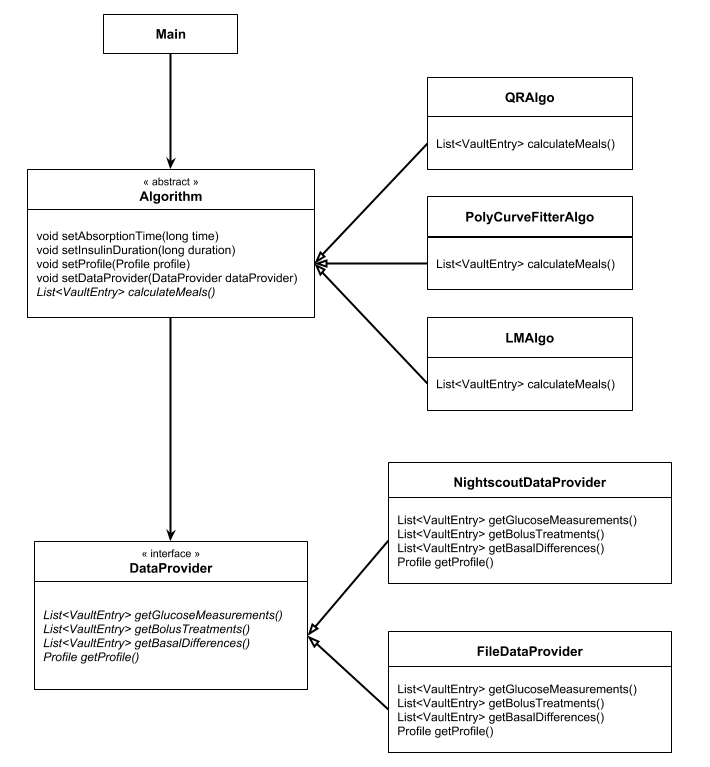
\includegraphics[width=1\textwidth]{UMLAlgos.png}

\newpage
\section*{Ablauf Mahlzeitenerkennung:}
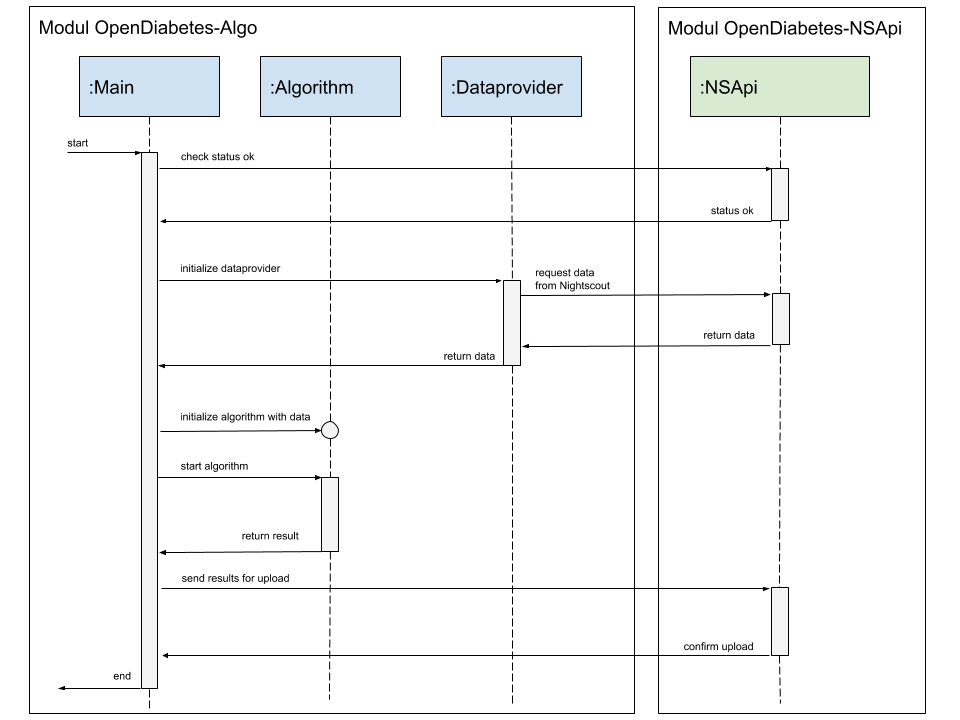
\includegraphics[width=1\textwidth]{SequenzdiagrammAlgorithmus.png}

\newpage
\section*{Ablauf synchronizieren von Daten:}
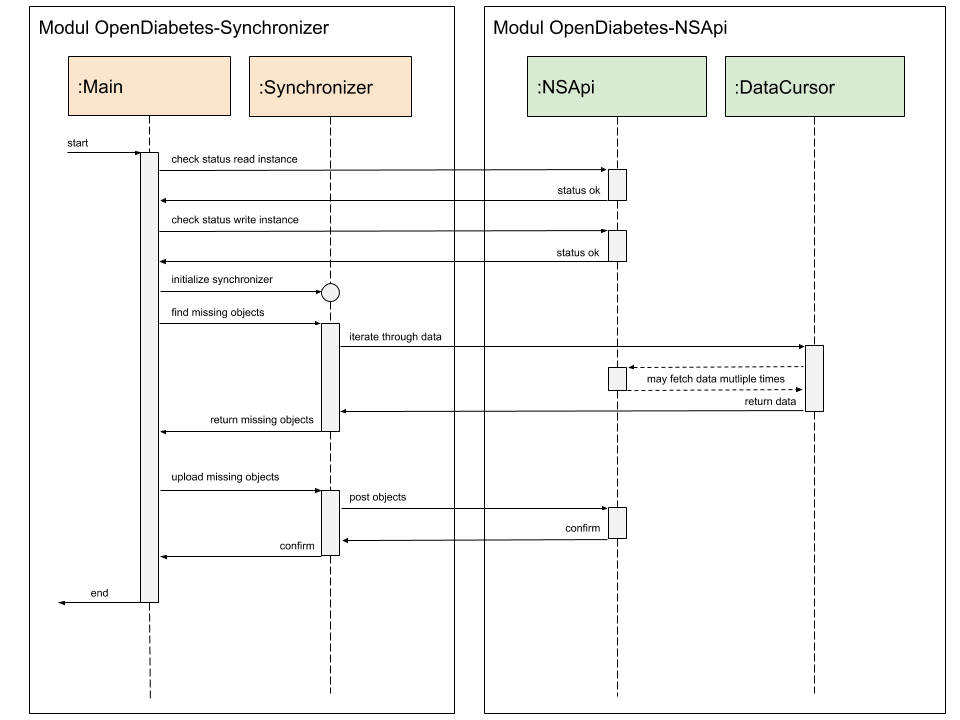
\includegraphics[width=1\textwidth]{SequenzdiagrammSynchronizer.png}


	

 \chapter{Anforderungen}
	\section{funktional}
\begin{itemize}
	\item Der Algorithmus muss die Größe der stattfindenden Mahlzeiten (Kohlenhydrate in Gramm) korrekt erkennen. 
	 Überprüft wird das an dem gegebenem Datensatz, auf Abschnitten in denen über einen Zeitraum von mindestens 6 Stunden durchgehend Blutzuckerdaten vorhanden sind. In diesen fanden alle 5 Minuten Messungen statt. Da die zu erkennenden Mahlzeiten nicht markiert sind, und dadurch ein direkter Vergleich nicht möglich ist, wird ein Blutzuckerverlauf anhand der bekannten Events und der berechneten Mahlzeiten generiert. Dieser soll zu jedem Zeitpunkt höchstens 10\% von dem originalen Blutzuckerverlauf abweichen. Eine höhere Abweichung wird toleriert, wenn der Abschnitt eindeutig seltsames Verhalten aufweist, z.B. einen plötzlichen Einbruch des Blutzuckerspiegels.
	
\item Der Synchronizer muss zwei Nightscout Insztanzen vergleichen und alle Einträge aus dem ersten, die aus dem zweiten fehlen, in das zweite einfügen.

\item Verschiedene Datenquellen müssen einbindbar sein. Lesen aus Nightscout oder einer Datei soll unterstützt sein.

\item Der Parser soll Nightscout Daten im JSON Format auf einheitliche, vom Arbeitgeber vorgegebene, Datentypen abbilden.



\item Darstellung der Daten/Mahlzeiten in Nightscout siehe User-Stories

\end{itemize}

	
	\section{nicht-funktional}
\begin{itemize}
	\item Das Programm muss auf einem PI Zero in angemessener Zeit laufen. Angemessen bedeutetd dabei unter 5 Minuten. 
	\begin{itemize}
	\item Anmerkung: Da uns kein PI Zero zur Verfügung steht, und der Arbeitgeber nicht allzu großen Wert darauf legt, wird diese Anforderung während des Projektes fallen gelassen. 
	\end{itemize}
	
\end{itemize}

{\let\clearpage\relax	\chapter{Qualitätssicherung}}

	Siehe QS-Dokument.

	\begin{comment}
{\let\clearpage\relax	\chapter{Risikomanagement}}

notwendig?  \textbf{{\large TODO}}
\end{comment}
	
{\let\clearpage\relax	\chapter{Rechtliches}}
	
	Wir entwickeln unter der AGPLv3-Lizenz und verwenden nur Open-Source Quellen. Dadurch vermeiden wir Copy-Right-Verletzungen und schließen jede Garantie an unserem Code aus.
	
\end{document}
